% Options for packages loaded elsewhere
\PassOptionsToPackage{unicode}{hyperref}
\PassOptionsToPackage{hyphens}{url}
\PassOptionsToPackage{dvipsnames,svgnames,x11names}{xcolor}
%
\documentclass[
  a4paper,
]{article}

\usepackage{amsmath,amssymb}
\usepackage{iftex}
\ifPDFTeX
  \usepackage[T1]{fontenc}
  \usepackage[utf8]{inputenc}
  \usepackage{textcomp} % provide euro and other symbols
\else % if luatex or xetex
  \usepackage{unicode-math}
  \defaultfontfeatures{Scale=MatchLowercase}
  \defaultfontfeatures[\rmfamily]{Ligatures=TeX,Scale=1}
\fi
\usepackage{lmodern}
\ifPDFTeX\else  
    % xetex/luatex font selection
\fi
% Use upquote if available, for straight quotes in verbatim environments
\IfFileExists{upquote.sty}{\usepackage{upquote}}{}
\IfFileExists{microtype.sty}{% use microtype if available
  \usepackage[]{microtype}
  \UseMicrotypeSet[protrusion]{basicmath} % disable protrusion for tt fonts
}{}
\makeatletter
\@ifundefined{KOMAClassName}{% if non-KOMA class
  \IfFileExists{parskip.sty}{%
    \usepackage{parskip}
  }{% else
    \setlength{\parindent}{0pt}
    \setlength{\parskip}{6pt plus 2pt minus 1pt}}
}{% if KOMA class
  \KOMAoptions{parskip=half}}
\makeatother
\usepackage{xcolor}
\usepackage[paperwidth=8.00in,paperheight=10.00in,left=1.25in,textwidth=
5.25in,top=1.00in,textheight=8.25in]{geometry}
\setlength{\emergencystretch}{3em} % prevent overfull lines
\setcounter{secnumdepth}{5}
% Make \paragraph and \subparagraph free-standing
\ifx\paragraph\undefined\else
  \let\oldparagraph\paragraph
  \renewcommand{\paragraph}[1]{\oldparagraph{#1}\mbox{}}
\fi
\ifx\subparagraph\undefined\else
  \let\oldsubparagraph\subparagraph
  \renewcommand{\subparagraph}[1]{\oldsubparagraph{#1}\mbox{}}
\fi


\providecommand{\tightlist}{%
  \setlength{\itemsep}{0pt}\setlength{\parskip}{0pt}}\usepackage{longtable,booktabs,array}
\usepackage{calc} % for calculating minipage widths
% Correct order of tables after \paragraph or \subparagraph
\usepackage{etoolbox}
\makeatletter
\patchcmd\longtable{\par}{\if@noskipsec\mbox{}\fi\par}{}{}
\makeatother
% Allow footnotes in longtable head/foot
\IfFileExists{footnotehyper.sty}{\usepackage{footnotehyper}}{\usepackage{footnote}}
\makesavenoteenv{longtable}
\usepackage{graphicx}
\makeatletter
\def\maxwidth{\ifdim\Gin@nat@width>\linewidth\linewidth\else\Gin@nat@width\fi}
\def\maxheight{\ifdim\Gin@nat@height>\textheight\textheight\else\Gin@nat@height\fi}
\makeatother
% Scale images if necessary, so that they will not overflow the page
% margins by default, and it is still possible to overwrite the defaults
% using explicit options in \includegraphics[width, height, ...]{}
\setkeys{Gin}{width=\maxwidth,height=\maxheight,keepaspectratio}
% Set default figure placement to htbp
\makeatletter
\def\fps@figure{htbp}
\makeatother
% definitions for citeproc citations
\NewDocumentCommand\citeproctext{}{}
\NewDocumentCommand\citeproc{mm}{%
  \begingroup\def\citeproctext{#2}\cite{#1}\endgroup}
\makeatletter
 % allow citations to break across lines
 \let\@cite@ofmt\@firstofone
 % avoid brackets around text for \cite:
 \def\@biblabel#1{}
 \def\@cite#1#2{{#1\if@tempswa , #2\fi}}
\makeatother
\newlength{\cslhangindent}
\setlength{\cslhangindent}{1.5em}
\newlength{\csllabelwidth}
\setlength{\csllabelwidth}{3em}
\newenvironment{CSLReferences}[2] % #1 hanging-indent, #2 entry-spacing
 {\begin{list}{}{%
  \setlength{\itemindent}{0pt}
  \setlength{\leftmargin}{0pt}
  \setlength{\parsep}{0pt}
  % turn on hanging indent if param 1 is 1
  \ifodd #1
   \setlength{\leftmargin}{\cslhangindent}
   \setlength{\itemindent}{-1\cslhangindent}
  \fi
  % set entry spacing
  \setlength{\itemsep}{#2\baselineskip}}}
 {\end{list}}
\usepackage{calc}
\newcommand{\CSLBlock}[1]{\hfill\break\parbox[t]{\linewidth}{\strut\ignorespaces#1\strut}}
\newcommand{\CSLLeftMargin}[1]{\parbox[t]{\csllabelwidth}{\strut#1\strut}}
\newcommand{\CSLRightInline}[1]{\parbox[t]{\linewidth - \csllabelwidth}{\strut#1\strut}}
\newcommand{\CSLIndent}[1]{\hspace{\cslhangindent}#1}

\makeatletter
\@ifpackageloaded{tcolorbox}{}{\usepackage[skins,breakable]{tcolorbox}}
\@ifpackageloaded{fontawesome5}{}{\usepackage{fontawesome5}}
\definecolor{quarto-callout-color}{HTML}{909090}
\definecolor{quarto-callout-note-color}{HTML}{0758E5}
\definecolor{quarto-callout-important-color}{HTML}{CC1914}
\definecolor{quarto-callout-warning-color}{HTML}{EB9113}
\definecolor{quarto-callout-tip-color}{HTML}{00A047}
\definecolor{quarto-callout-caution-color}{HTML}{FC5300}
\definecolor{quarto-callout-color-frame}{HTML}{acacac}
\definecolor{quarto-callout-note-color-frame}{HTML}{4582ec}
\definecolor{quarto-callout-important-color-frame}{HTML}{d9534f}
\definecolor{quarto-callout-warning-color-frame}{HTML}{f0ad4e}
\definecolor{quarto-callout-tip-color-frame}{HTML}{02b875}
\definecolor{quarto-callout-caution-color-frame}{HTML}{fd7e14}
\makeatother
\makeatletter
\@ifpackageloaded{bookmark}{}{\usepackage{bookmark}}
\makeatother
\makeatletter
\@ifpackageloaded{caption}{}{\usepackage{caption}}
\AtBeginDocument{%
\ifdefined\contentsname
  \renewcommand*\contentsname{Table of contents}
\else
  \newcommand\contentsname{Table of contents}
\fi
\ifdefined\listfigurename
  \renewcommand*\listfigurename{List of Figures}
\else
  \newcommand\listfigurename{List of Figures}
\fi
\ifdefined\listtablename
  \renewcommand*\listtablename{List of Tables}
\else
  \newcommand\listtablename{List of Tables}
\fi
\ifdefined\figurename
  \renewcommand*\figurename{Figure}
\else
  \newcommand\figurename{Figure}
\fi
\ifdefined\tablename
  \renewcommand*\tablename{Table}
\else
  \newcommand\tablename{Table}
\fi
}
\@ifpackageloaded{float}{}{\usepackage{float}}
\floatstyle{ruled}
\@ifundefined{c@chapter}{\newfloat{codelisting}{h}{lop}}{\newfloat{codelisting}{h}{lop}[chapter]}
\floatname{codelisting}{Listing}
\newcommand*\listoflistings{\listof{codelisting}{List of Listings}}
\makeatother
\makeatletter
\makeatother
\makeatletter
\@ifpackageloaded{caption}{}{\usepackage{caption}}
\@ifpackageloaded{subcaption}{}{\usepackage{subcaption}}
\makeatother
\newcounter{quartocallouttipno}
\newcommand{\quartocallouttip}[1]{\refstepcounter{quartocallouttipno}\label{#1}}
\ifLuaTeX
  \usepackage{selnolig}  % disable illegal ligatures
\fi
\usepackage{bookmark}

\IfFileExists{xurl.sty}{\usepackage{xurl}}{} % add URL line breaks if available
\urlstyle{same} % disable monospaced font for URLs
\hypersetup{
  pdftitle={Artigo à Prova de Futuro},
  colorlinks=true,
  linkcolor={blue},
  filecolor={Maroon},
  citecolor={Blue},
  urlcolor={Blue},
  pdfcreator={LaTeX via pandoc}}

\title{Artigo à Prova de Futuro}
\usepackage{etoolbox}
\makeatletter
\providecommand{\subtitle}[1]{% add subtitle to \maketitle
  \apptocmd{\@title}{\par {\large #1 \par}}{}{}
}
\makeatother
\subtitle{Jornada de Open Science na Prática}
\author{}
\date{}

\begin{document}
\maketitle

\bookmarksetup{startatroot}

\section*{Home 🏢}\label{sec-home}

\markboth{Home 🏢}{Home 🏢}

Página do curso \textbf{``Artigo à Prova de Futuro: Jornada de Open
Science na Prática''}. Aqui você encontrará informações sobre o programa
do curso, materiais para seu acompanhamento e sugestões de leituras
sobre a prática da ciência aberta (artigos, notas de aulas, blogs,
vídeos, etc.).

Caso você caiu nessa página por acaso (🤣😁😉), saiba que o poderá se
inscrever no curso \href{https://forms.gle/b6Zio7oL8XxxhhtS9}{aqui}:
independente se ele estiver acontecendo no momento, será convidado a
participar da próxima versão.

\subsection*{Sobre os instrutores}\label{sec-instrutor}

\markright{Sobre os instrutores}

O curso é coordenado e ministrado por Pablo Rogers, doutor em
administração pela Universidade de São Paulo (FEA/USP) e professor de
finanças e métodos quantitativos desde 2005. Em sua
\href{https://github.com/phdpablo}{página de perfil do Github} temos
informações de seus trabalhos recentes, e no seu
\href{https://phdpablo.com/}{site pessoal}, detalhes sobre suas
formações, competências, trajetória e projetos.

Na sua versão atual o curso também será ministrado por Ricardo Limongi,
doutor em administração pela Fundação Getúlio Vargas (FGV-SP) e
professor de marketing e métodos quantitativos desde 2008 e atual editor
chefe da Brazilian Administration Review (BAR). Em seu
\href{https://www.instagram.com/limongi/}{perfil do Instagram} é
possível acompanhar sua agenda de atividades, cursos e palestras sobre
inteligência artificial aplicada aos negócios e pesquisa. Em seu
\href{https://www.youtube.com/@ricardolimongi_ia}{canal do YouTube}, é
possível encontrar vídeos das suas atividades: congressos, palestras,
aulas, etc.

\subsection*{Sobre o curso}\label{sec-about}

\markright{Sobre o curso}

O curso tem objetivo de introduzir os conceitos relacionados com a
ciência aberta e a prática da pesquisa reprodutível. O curso aborda
temas introdutórios sobre ciência aberta, com foco no ferramental
disponível para tornar a pesquisa mais transparente, reprodutível e
acessível. O curso é voltado para pesquisadores e estudantes de
pós-graduação, mas aberto a qualquer pessoa interessada em aprender
sobre a prática da ciência aberta. O protagonista do curso é o
pesquisador brasileiro que deseja aprimorar a qualidade e a
transparência de sua pesquisa, e que busca ferramentas para tornar-lá
mais eficiente e acessível.

Trata-se de um curso intermitente programado para acontecer em 4
encontros de 4 horas/aula (ou 8 encontros de 2 horas/aula), totalizando
16 horas/aula. Num primeiro momento, a ideia que o curso seja remoto e
síncrono para alcançar um número maior de interessados. Ele poderá
acontecer mais de uma vez no ano, com datas e horários a serem
definidos. Para o calendário atual do curso, consulte a seção
\href{https://phdpablo.github.io/curso-open-science/00-schedule.html}{Agenda}.

O curso é gratuito e com de certificado de extensão pela Universidade
Federal de Uberlândia (UFU). As inscrições são feitas por meio de um
\href{https://forms.gle/wRNWAU9Ffyp7o4Vq9}{formulário} intermediado pelo
projeto
\href{https://www.youtube.com/c/PsicoEconoMETRIA}{Psico\&Econo\_METRIA}.
Quando da previsão das datas, uma campanha de e-mail marketing divulgará
o link para a inscrição através de coordenações de pós-graduações
selecionadas.

As vagas são limitadas e a seleção será feita por ordem de inscrição.
Após o preenchimento das vagas, os demais interessados serão inscritos
automaticamente numa lista de espera e, tempestivamente, serão avisados
sobre a próxima edição do curso. Após selecionados, os inscritos
receberão um e-mail com instruções para acesso à plataforma de aulas
síncronas e para a realização das atividades prévias ao curso.

\subsection*{Ementa do curso}\label{sec-ementa}

\markright{Ementa do curso}

Introdução da Ciência Aberta / Repositórios da Ciência Aberta /
Gerenciamento de Referências e Bibliotecas / Gestão de Dados e Projetos
/ Controle de Versão / Documentos Reprodutíveis / Controle de Ambiente
(containers) / IA Aplicada à Pesquisa Científica.

\subsection*{Metodologia}\label{sec-method}

\markright{Metodologia}

Num primeiro momento, o curso foi concebido para acontecer de forma
remota e síncrona, com aulas expositivas e teóricas, porém em grande
medida, o conteúdo é essencialmente prático. Algumas aulas poderão ser
gravadas e disponibilizadas no
\href{https://www.youtube.com/c/PsicoEconoMETRIA}{canal do YouTube do
projeto Psico\&Econo\_METRIA}, mas a intenção é que o conteúdo principal
seja síncrono, para uma maior interação entre os participantes.

Nesse sentido, o material do curso organizado nessa página refere-se ao
roteiro estruturado de tudo que se vê nas aulas síncronas e conteúdos
adicionais (bibliografia, notas de aulas, links, etc).

A proposta do curso busca seguir de perto a mensagem de Dogucu and
Çetinkaya-Rundel (2022). Nesse artigo as autoras abordam a importância
da reprodutibilidade na ciência de dados, tanto na pesquisa quanto no
ensino. Elas recomendam que os professores-pesquisadores adotem fluxos
de trabalho reprodutíveis em suas pesquisas e ensinem esses fluxos de
trabalho aos seus alunos. Elas propõem uma dimensão para as práticas de
reprodutibilidade, focada exclusivamente nas ferramentas para o ensino
(todos os materiais de ensino devem ser computacionalmente
reprodutíveis, bem documentados e abertos).

Artigo à Prova de Futuro: Jornada de Open Science na Prática by Pablo
Rogers is licensed under CC BY-NC-SA 4.0

\bookmarksetup{startatroot}

\section*{Pré-requisitos 📇}\label{sec-prework}

\markboth{Pré-requisitos 📇}{Pré-requisitos 📇}

O curso não exige conhecimento prévio em programação, mas é recomendável
que o aluno tenha familiaridade com o uso de computadores (ambiente
Windows) e com a escrita de textos científicos. Nesse sentido, não é
necessário ter conhecimento prévio sobre as ferramentas e plataformas
que utilizaremos no curso: Zotero, OSF, Zenodo, Git, Github, RStudio,
Quarto/RMarkdown, Docker, etc; mas desejável que o aluno já as tenha
instalado e/ou cadastro nas plataformas.

Abaixo eu descrevo sucintamente o que é cada uma dessas ferramentas e
plataformas, e como você pode se preparar para o curso. Também apresento
um vídeo curto sobre a instalação e cadastro em cada uma delas. A ideia
é que você já tenha todas as ferramentas e plataformas instaladas e/ou
cadastro antes do início do curso, para que possamos focar no conteúdo e
prática durante as aulas síncronas. Mas pode ficar tranquilo, pois na
primeira aula do curso abordaremos essas tarefas, e caso ainda haja
alguma dúvida na instalação e cadastro, dedicaremos algum tempo para
saná-las.

Outras soluções que iremos discutir e testar durante o curso, como
alguns pacotes do R, e aplicações de IA no último módulo, deixaremos
para as aulas remotas. Essas soluções na sua maioria requerem cadastros
rápidos, e podem ser feitos de forma instantânea via conta
Google/Microsoft/Apple.

\begin{tcolorbox}[enhanced jigsaw, left=2mm, arc=.35mm, rightrule=.15mm, opacitybacktitle=0.6, breakable, toprule=.15mm, bottomrule=.15mm, leftrule=.75mm, colframe=quarto-callout-important-color-frame, coltitle=black, bottomtitle=1mm, titlerule=0mm, toptitle=1mm, title=\textcolor{quarto-callout-important-color}{\faExclamation}\hspace{0.5em}{Tip \ref*{tip-prompt}: ChatGPT para suas notas de leituras}, opacityback=0, colbacktitle=quarto-callout-important-color!10!white, colback=white]

\quartocallouttip{tip-prompt} 

Os resumos das bibliografias que apresento em cada uma das seções foram
elaborados com o auxílio do ChatGPT 4, seja pelo o
\href{https://chat.openai.com/}{webapp da OpenAI} ou pelo
\href{https://copilot.microsoft.com/}{Copilot} (ou buscador Bing) da
Microsoft.

Eu destaco (seleciono através de marca texto no Zotero, por exemplo) as
passagens que considero importante do artigo científico, tendo em vista
a minha perspectiva e fins no momento da leitura, e posteriormente copio
e colo as notas de leitura com a seguinte prompt:

``\emph{Senteces in the text are reading notes, that is, what I found
most important and interesting, from a scientific article on the topic
open science. I would like you to summarize the notes in a descriptive
text and concatenate the arguments highlighted in the notes. Give your
answer in Portuguese}''

\end{tcolorbox}

\begin{tcolorbox}[enhanced jigsaw, left=2mm, arc=.35mm, rightrule=.15mm, opacitybacktitle=0.6, breakable, toprule=.15mm, bottomrule=.15mm, leftrule=.75mm, colframe=quarto-callout-caution-color-frame, coltitle=black, bottomtitle=1mm, titlerule=0mm, toptitle=1mm, title=\textcolor{quarto-callout-caution-color}{\faFire}\hspace{0.5em}{Não confie cegamente na IA}, opacityback=0, colbacktitle=quarto-callout-caution-color!10!white, colback=white]

Eu simplesmente copiei e colei os resultados do ChatGPT para compilar
essas notas de leituras? Não. Após o resultado do ChatGPT eu reviso o
sumário das notas de leituras e faço ajustes, que somente são possíveis
porque li o artigo por completo. A despeito do ChatGPT fazer um bom
serviço nesse sentido, ele ainda comete muitos deslizes. Deslizes esses
que você não pode deixar passar num texto científico, e somente captaria
a partir da leitura do artigo ou sendo conhecedor do assunto abordado.

\end{tcolorbox}

\begin{tcolorbox}[enhanced jigsaw, left=2mm, arc=.35mm, rightrule=.15mm, opacitybacktitle=0.6, breakable, toprule=.15mm, bottomrule=.15mm, leftrule=.75mm, colframe=quarto-callout-note-color-frame, coltitle=black, bottomtitle=1mm, titlerule=0mm, toptitle=1mm, title=\textcolor{quarto-callout-note-color}{\faInfo}\hspace{0.5em}{Outra curiosidade\ldots{}}, opacityback=0, colbacktitle=quarto-callout-note-color!10!white, colback=white]

A
\href{https://phdpablo.github.io/curso-open-science/img/cover.png}{imagem
cover desse curso} foi gerada por uma IA, com posteriores ajustes (off
course!). Existem diversos geradores de imagens que você pode testar
gratuitamente, mas eu costumo utilizar o i)
\href{https://openai.com/dall-e/}{DALL-E}, que é uma solução da OpenAI
que também pode ser utilizada no
\href{https://copilot.microsoft.com/}{Copilot da Microsoft}; ii) o
\href{https://playgroundai.com/}{PlaygroundAI}, e iii) o
\href{https://gemini.google.com/app}{Gemini} do Google.

\end{tcolorbox}

\subsection*{Github}\label{sec-githubprework}
\addcontentsline{toc}{subsection}{Github}

\markright{Github}

Primeiramente, se cadastre no Github: \url{https://github.com/signup},
pois com ele você poderá acessar o material do curso e interagir com os
demais participantes. E com a conta do Github você também poderá se
cadastrar em outras plataformas, como o Zenodo, OSF, etc. Algumas
features que aprenderemos no curso exigem o vínculo entre as contas. Se
for professor ou estudante, você pode solicitar o
\href{https://education.github.com/}{GitHub Education} e ter acesso, por
exemplo, ao Copilot, uma das ferramentas de IA que abordaremos no último
módulo. Por isso, é importante que você se cadastre com um e-mail
institucional. Use o mesmo e-mail para se cadastrar em todas
plataformas.

\url{https://youtu.be/Nmjh9KsV6eU}

\subsection*{Git}\label{sec-gitprework}
\addcontentsline{toc}{subsection}{Git}

\markright{Git}

Github não é a mesma coisa que Git. O Github é uma plataforma, e o Git é
uma ferramenta. Instale a versão mais recente do Git:
\url{https://git-scm.com/downloads}. O Git é uma ferramenta de controle
de versão, e o Github é uma plataforma que utiliza o Git. O Git é uma
ferramenta essencial para a prática da ciência aberta, e é uma das
ferramentas mais importantes para o pesquisador que deseja tornar sua
pesquisa mais transparente e reprodutível.

\url{https://youtu.be/XCa6mE0bEI0}

\subsection*{Zotero}\label{sec-zoteroprework}
\addcontentsline{toc}{subsection}{Zotero}

\markright{Zotero}

Baixe a versão mais recente do Zotero:
\url{https://www.zotero.org/download/} e cadastre uma conta:
\url{https://www.zotero.org/user/register/}. Vamos discutir sobre o
Zotero e diversos plugins que são úteis no dia-a-dia do pesquisador.
Atualmente, o Zotero é a ferramenta mais completa para gerenciamento de
referências e bibliotecas, e se integra nativamente com o RStudio.

\url{https://youtu.be/ZSFq6LHaDJ4}

\subsection*{OSF}\label{sec-osfprework}
\addcontentsline{toc}{subsection}{OSF}

\markright{OSF}

Cadastre no Open Science Framework (OSF):
\url{https://osf.io/register/}. Como veremos, essa plataforma é uma das
mais importantes para a prática da ciência aberta. Ela está no começo
(pré-registro) e no final (repositório de dados e pré-print) do ciclo de
vida (workflow) de um projeto de pesquisa.

\url{https://youtu.be/WQ4O-8O6MwI}

\subsection*{Zenodo}\label{sec-zenodoprework}
\addcontentsline{toc}{subsection}{Zenodo}

\markright{Zenodo}

Apesar do Zenodo cumprir funções similares ao OSF e até mesmo ao Github,
ele é mais voltado para a publicação de dados e publicações científicas.
Cadastre no Zenodo: \url{https://zenodo.org/login/} e víncule sua conta
com o Github. Isso será útil, principalmente, para geração de DOI de
repositórios do Github.

\url{https://youtu.be/pZaqL3Auxb0}

\subsection*{RStudio}\label{sec-rstudioprework}
\addcontentsline{toc}{subsection}{RStudio}

\markright{RStudio}

Baixe a versão mais recente do RStudio:
\url{https://posit.co/download/rstudio-desktop/}. O RStudio é uma
Integrated Development Environment (IDE) para a linguagem R. O RStudio é
uma ferramenta essencial para a prática da ciência aberta em R, pois
integra as principais soluções que abordaremos no curso (Zotero, Quarto,
Git/Github, etc.). A empresa RStudio recentemente mudou o nome para
Posit, com o objetivo refletir melhor a expansão da empresa para além do
desenvolvimento de ferramentas para R, incluindo Python e outras
linguagens. Nesse mesmo link você pode baixar o R, que é a linguagem de
programação que utilizaremos no curso.

\url{https://youtu.be/KM2jxaNIEUk}

\subsection*{Quarto}\label{sec-quartoprework}
\addcontentsline{toc}{subsection}{Quarto}

\markright{Quarto}

Baixe a versão mais recente do Quarto: \url{https://www.quarto.org/}. O
Quarto é uma linguagem de marcação que permite a criação de documentos
reprodutíveis e dinâmicos. Ele é uma evolução e tende a substituir o
RMarkdown, que é a principal linguagem de marcação do R. O Quarto
engloba e adiciona diversas outras vantagens ao RMarkdown, tal como a
possibilidade de criar documentos reprodutíveis em Python, Julia, etc.
Se você já tem algum conhecimento de RMarkdown, não se preocupe, pois o
Quarto é uma extensão natural.

\url{https://youtu.be/-HvOMVkk6I4}

\subsection*{Docker}\label{sec-dockerprework}
\addcontentsline{toc}{subsection}{Docker}

\markright{Docker}

Baixe a versão mais recente do Docker:
\url{https://www.docker.com/products/docker-desktop}. Nesse mesmo link
você cria uma conta. O Docker é uma plataforma para desenvolvimento,
envio e execução de aplicativos. O Docker é uma ferramenta essencial
para a prática da ciência aberta, pois permite a criação de ambientes
reprodutíveis.

\url{https://youtu.be/WjXQxhTLlrQ}

\bookmarksetup{startatroot}

\section*{Agenda 📅}\label{sec-schedule}

\markboth{Agenda 📅}{Agenda 📅}

Planejamento dos dias (📅) e horários das aulas (⏲️), conforme a ementa
do curso. Na seção de cada uma das aulas temos materiais adicionais para
o respectivo conteúdo. Quando disponível, por aqui, poderás acessar os
slides utilizados nas aulas (🗣️), aulas gravadas ou indicações de vídeo
(🎥)\footnote{Na primeira edição do curso a equipe organizadora decidiu
  não publicar as aulas. Elas estarão disponíveis apenas privativamente
  para os inscritos no curso, através da platorma de reuniões adotada
  (Microsoft Teams). No futuro, quando o coordenador considerar que o
  curso esteja efetivamente formatado, as aulas gravadas serão
  publicadas no canal
  \href{https://www.youtube.com/c/PsicoEconoMETRIA}{Psico\&Econo\_METRIA}}
e leituras básica sobre os conteúdos (📓).

\begin{longtable}[]{@{}
  >{\raggedright\arraybackslash}p{(\columnwidth - 6\tabcolsep) * \real{0.1507}}
  >{\centering\arraybackslash}p{(\columnwidth - 6\tabcolsep) * \real{0.1507}}
  >{\centering\arraybackslash}p{(\columnwidth - 6\tabcolsep) * \real{0.5479}}
  >{\centering\arraybackslash}p{(\columnwidth - 6\tabcolsep) * \real{0.1507}}@{}}
\toprule\noalign{}
\begin{minipage}[b]{\linewidth}\raggedright
Aula/Conteúdo
\end{minipage} & \begin{minipage}[b]{\linewidth}\centering
Data
\end{minipage} & \begin{minipage}[b]{\linewidth}\centering
Material Principal
\end{minipage} & \begin{minipage}[b]{\linewidth}\centering
Instrutor
\end{minipage} \\
\midrule\noalign{}
\endhead
\bottomrule\noalign{}
\endlastfoot
Chapter~\ref{sec-intro} & 📅04/06/24⏲️19:00 &
\href{./resources/01-intro.pptx}{🗣}\href{https://www.youtube.com/live/7ewEcTATkZM?si=Lq40IAoDgsy_A619}{🎥}\href{https://doi.org/10.1590/S0034-759020230408}{📓}
& Ricardo Limongi \\
Chapter~\ref{sec-osf} & 📅06/06/24⏲️19:00 &
\href{https://osf.io/wm8vs}{🗣️}\href{https://www.youtube.com/watch?v=B19MPDJX_vs}{🎥}\href{https://doi.org/10.1002/cpet.32}{📓}
& Pablo Rogers \\
Chapter~\ref{sec-zotero} & 📅11/06/24⏲️19:00 & 🗣️🎥📓 & Pablo Rogers \\
Chapter~\ref{sec-project} & 📅13/06/24⏲️19:00 & 🗣️🎥📓 & Pablo Rogers \\
Chapter~\ref{sec-git} & 📅18/06/24⏲️19:00 & 🗣️🎥📓 & Pablo Rogers \\
Chapter~\ref{sec-quarto} & 📅20/06/24⏲️19:00 & 🗣️🎥📓 & Pablo Rogers \\
Chapter~\ref{sec-docker} & 📅25/06/24⏲️19:00 & 🗣️🎥📓 & Pablo Rogers \\
Chapter~\ref{sec-AI} & 📅27/06/24⏲️19:00 & 🗣️🎥📓 & Ricardo Limongi \\
\end{longtable}

\bookmarksetup{startatroot}

\section{Introdução à Ciência Aberta}\label{sec-intro}

A pesquisa científica atual\footnote{O texto apresentado nessa seção é
  uma compilação de fragmentos do Projeto APQ-01225-24 submetido ao
  Edital Nº 001/2024 - Demanda Universal, da FAPEMIG, ainda em análise.
  O detalhamento desse projeto, quando se tornar público, poderá ser
  acompanhado no \href{http://osf.io/dnrgf}{OSF}: Rogers, P., Limongi,
  R., \& Barboza, F. (2024, May 29). The Practice of Open Science in
  Brazil. Retrieved from osf.io/dnrgf} enfrenta vários desafios (Munafò
et al. 2017). Problemas como o pequeno tamanho da amostra, pequenos
tamanhos de efeito, p-hacking e HARKing (viés positivo de publicação),
conflitos de interesse e a competição entre cientistas que trabalham
isoladamente sem combinar seus esforços, têm sido apontados como
catalizadores do que se convencionou chamar de ``crise de
reprodutibilidade'' na ciência (M. Baker 2016; Munafò et al. 2017).

Pesquisas apontam que mais de 70\% de pesquisadores que tentaram,
falharam em reproduzir os experimentos de outros cientistas, e mais da
metade falhou em reproduzir seus próprios experimentos (M. Baker 2016),
com estimativa de que 85\% dos esforços de pesquisas estejam sendo
desperdiçados (Munafò et al. 2017), gerando custos econômicos
bilionários (Freedman, Cockburn, and Simcoe 2015).

A despeito daqueles que advogam que não existe essa tal ``crise de
reprodutibilidade'' (Bernard 2023; Fanelli 2018; Protzko et al. 2023), a
grande maioria da comunidade científica concorda com sua existência e
defende a melhoria da transparência, reprodutibilidade e eficiência na
ciência (M. Baker 2016).

Nesse contexto, o movimento da Ciência Aberta (CA) tem ganhado
notoriedade e mudado a percepção sobre o cenário científico global
(Crüwell et al. 2019). Ele busca tornar o conhecimento científico mais
acessível, transparente e colaborativo. Se apresenta como uma coleção de
práticas de democratização do conhecimento e ruptura com o formato único
de divulgação do conhecimento científico (Crüwell et al. 2019; Heinz and
Miranda 2024; Munafò et al. 2017). Ele surge do embate entre aqueles que
buscam compartilhar o conhecimento e aqueles que defendem mecanismos de
apropriação privada para a produção científica (Heinz and Miranda 2024).

A CA é um termo múltiplo e genérico (Vicente-Saez and Martinez-Fuentes
2018), que representa diversas interpretações, e é considerada um novo
modelo de divulgação e produção de resultados científicos por meio do
acesso livre e irrestrito ao conhecimento (Heinz and Miranda 2024). A CA
não é apenas um conceito, mas uma prática multifacetada que influencia o
ciclo de vida da pesquisa, desde a concepção até a disseminação dos
resultados (Silva and Silveira 2019).

Existem pelo menos cinco escolas de pensamento dentro da CA. Estas
escolas abrangem desde a arquitetura tecnológica necessária para
suportar a ciência até a inclusão do público geral na criação de
conhecimento, passando pela medição do impacto alternativo, acesso ao
conhecimento como um direito humano, e a pesquisa colaborativa como
inovação aberta (Silva and Silveira 2019).

A taxonomia proposta pela
\href{https://www.fosteropenscience.eu/foster-taxonomy/open-workflow-tools}{FOSTER}
(Facilitate Open Science Training for Eurpean Research), e sua releitura
revisada e ampliada para o contexto latino americano por Silveira et al.
(2023), tendo em vista as recomendações da UNESCO (2021), nos dá uma
dimensão da complexidade do assunto (vide ilustração em:
\url{https://doi.org/10.5281/zenodo.7836884}).

Existem vários argumentos que sustentam a importância da CA (Heinz and
Miranda 2024). Primeiramente, a CA pode trazer benefícios sociais
significativos, pois contribui para o avanço do conhecimento, a
inovação, a educação, a transparência e a participação cidadã. Além
disso, a CA pode trazer benefícios científicos ao aumentar a qualidade,
a reprodutibilidade, a eficiência e o impacto da pesquisa científica.
Ela também facilita a colaboração, a comunicação e a
interdisciplinaridade entre os pesquisadores. Por fim, a CA pode trazer
benefícios éticos ao promover a integridade, a responsabilidade, a
equidade e a diversidade na ciência, além de respeitar os direitos dos
autores, dos participantes e da sociedade como um todo.

Esses argumentos são fundamentais para legitimar a CA e destacar sua
importância no mundo atual (Heinz and Miranda 2024), principalmente,
como potencial transformador para reduzir desigualdades existentes em
tecnologias de informação e comunicação -- reduzir exclusões digitais,
tecnológicas e de conhecimento --, e acelerar o progresso rumo à
implementação da Agenda 2030 e realização dos Objetivos de
Desenvolvimento Sustentável (UNESCO 2021).

O movimento da CA no Brasil está em uma fase transitória (Rezende and
Falgueras 2020) -- ainda consolidando o acesso aberto -- com o governo
desempenhando um papel crucial nesse processo. O Brasil tem ganhado
destaque por sua abordagem única na implementação da CA. Esta abordagem
é moldada por marcos regulatórios que se estendem desde o governo até as
instituições e agências de financiamento. Os regulamentos brasileiros,
particularmente aqueles que promovem a abertura de dados governamentais,
têm um impacto direto na prática científica. Eles incentivam a
transparência e facilitam o acesso a dados científicos originados de
instituições públicas (Rezende and Falgueras 2020).

A trajetória brasileira rumo à CA inicia com a abertura de dados na
esfera governamental entre 2009 e 2016, evoluindo para a criação de um
grupo de trabalho em 2017 pelo Ministério da Ciência, Tecnologia,
Inovações e Comunicações (MCTIC) para desenvolver uma política nacional
para a CA. Este esforço concentrou ênfase no reconhecimento dos dados de
pesquisa como ativos de desenvolvimento científico, econômico e social,
buscando facilitar seu acesso, compartilhamento e reutilização (Rezende
and Falgueras 2020).

Talvez por esse motivo, as políticas institucionais brasileiras revelam
um cenário ainda muito influenciado pela ``via verde'' do movimento de
acesso aberto, caracterizado pelo depósito de dados em repositórios
digitais abertos, e que o comprometimento efetivo do Brasil com a CA
ainda é incipiente. As regulamentações atuais favorecem principalmente o
acesso aberto, sem abordar de maneira abrangente outros aspectos da CA
(Rezende and Falgueras 2020). O Brasil é um dos líderes mundiais no
fornecimento de acesso universal às suas pesquisas e estudos (Neto,
Willinsky, and Alperin 2016), com crescimento estável de sua produção
científica disponível em acesso aberto, principalmente, as áreas de
Agricultura e Ciência \& Tecnologia (Caballero-Rivero, Sánchez-Tarragó,
and Santos 2019).

Em termos de pesquisa acadêmica sobre o tema no Brasil, os estudos são
precoces e concentrados na área de Ciência da Informação (Albano,
Pedroso, and Caetano 2023). A despeito da maturidade da CA no Brasil, a
importância do tema -- materializada na quantidade de produção acadêmica
-- tem aumentado vertiginosamente (Albano, Pedroso, and Caetano 2023), e
a dispersão de autores e respectivas instituições que publicam sobre o
assunto, parece ser a situação predominante.

Apesar de importantes atores nacionais, tais como CAPES, CNPq e Scielo,
defenderem o crescimento de iniciativas de CA (Mendes-Da-Silva 2023), o
assunto no Brasil parece estar circunscrito em iniciativas de
importantes periódicos nacionais sobre dados aberto, capitaneados pelas
orientações da Scielo. Não foi encontrada nenhuma pesquisa empírica,
sobre a prática da CA no Brasil.

Por prática de CA entende-se a perspectiva micro da CA, relacionadas com
as terminologias e conhecimento em torno do fluxo de trabalho do gerador
de conhecimento científico aberto (Figure~\ref{fig-ca-micro}), ou seja,
o cientista que se propõe tornar sua pesquisa transparente, reprodutível
e replicável.

\begin{figure}

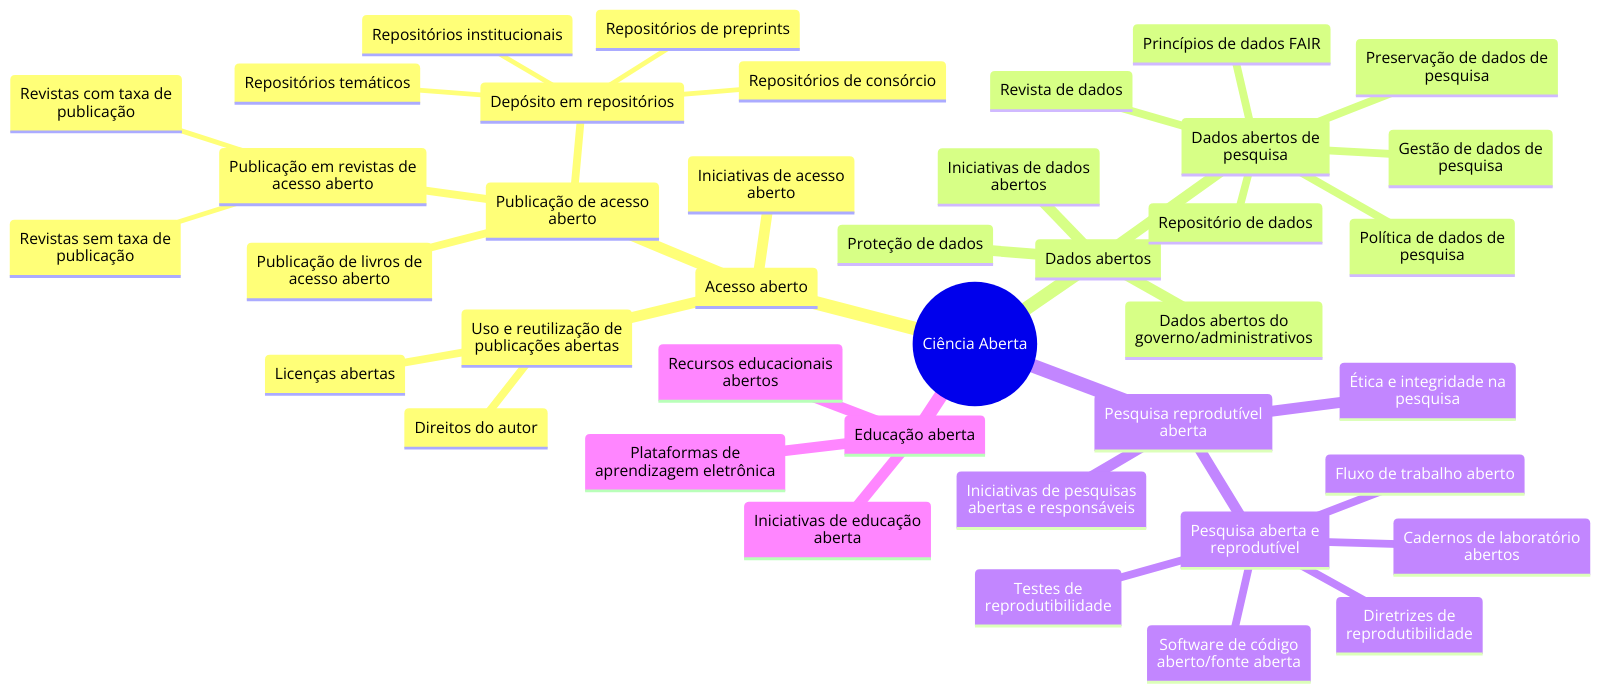
\includegraphics{img/ca-micro.png}

\caption{\label{fig-ca-micro}Perspectiva micro da CA. Taxonomia
relacionada com terminologias e conhecimento em torno da prática (fluxo
de trabalho) do gerador de conhecimento científico aberto. Ilustração
disponível em: \url{https://doi.org/10.5281/zenodo.10835001}.}

\end{figure}%

Exclui-se a perspectiva macro, relacionadas com as ramificações
conceituais da CA concernentes às políticas públicas, infraestrutura,
envolvimento aberto de atores sociais e diálogo aberto com outros
sistemas de conhecimento (Figure~\ref{fig-ca-macro}). Essa última
perspectiva está fora do escopo da discussão do curso, que se concentra
em algumas das dimensões da perspectiva micro, particularmente, as
ferramentas disponíveis para compilação dos produtos científicos que
integram a publicação científica (UNESCO 2021).

\begin{figure}

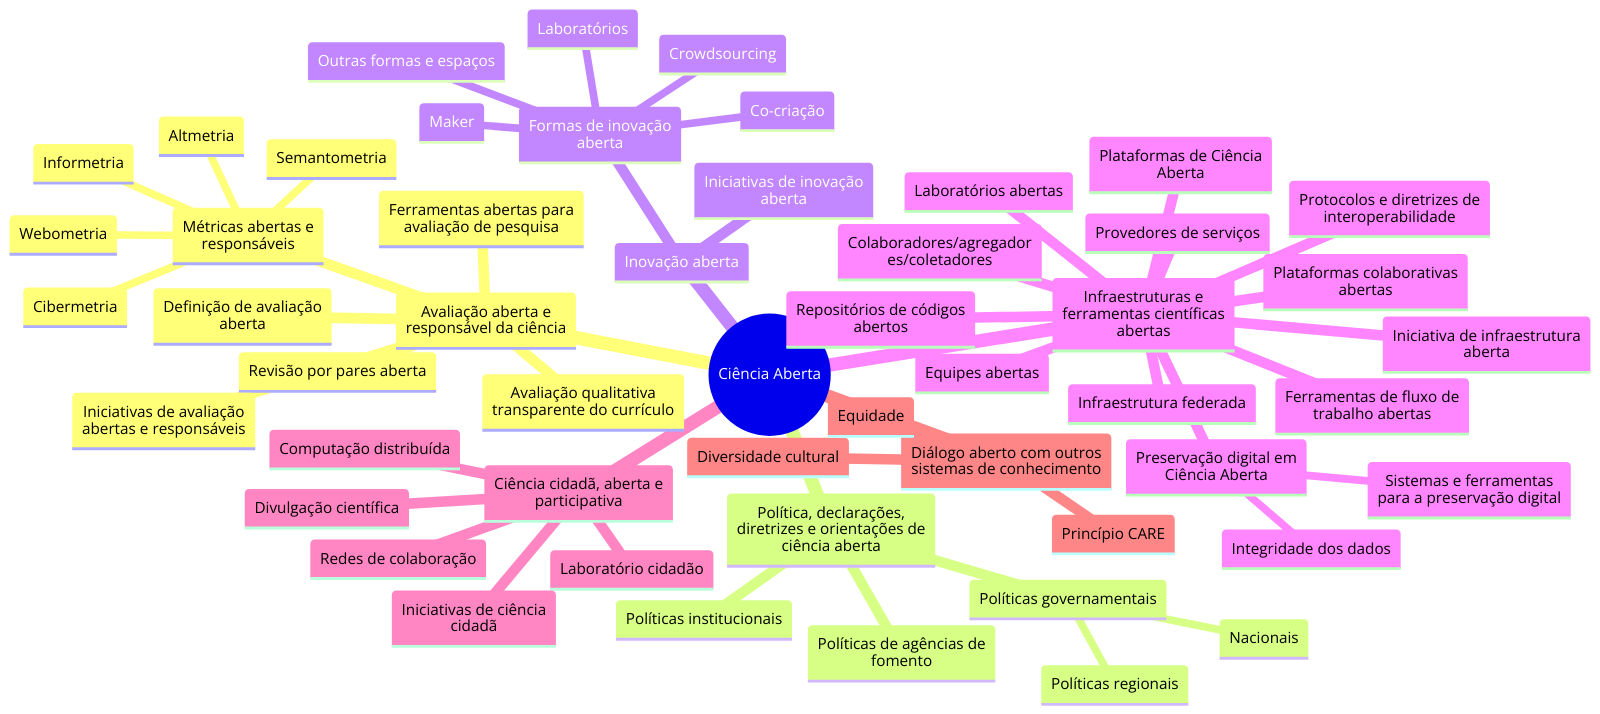
\includegraphics{img/ca-macro.png}

\caption{\label{fig-ca-macro}Perspectiva macro da CA. Taxonomia
relacionada com as ramificações conceituais da CA concernentes às
políticas (públicas), infraestrutura, envolvimento aberto de atores
sociais (sociedade) e diálogo aberto com outros sistemas de
conhecimento. Ilustração disponível em:
\url{https://doi.org/10.5281/zenodo.10835001}}

\end{figure}%

Apesar de uma verossímil expectativa desabonadora, tendo em vista o
contexto da CA no Brasil, o diagnóstico da situação da prática da CA se
mostra importante, \emph{per si}, pois:

\begin{enumerate}
\def\labelenumi{\arabic{enumi}.}
\item
  ajuda a compreender a natureza exata do problema, suas causas, efeitos
  e riscos;
\item
  auxilia a alocação eficiente de recursos pelos atores envolvidos
  (e.g., os programas de pós-graduação podem direcionar os recursos para
  onde eles são mais necessários e onde terão o maior impacto;
\item
  orienta indicadores de desempenho e metas realistas, o que facilita a
  avaliação do progresso e a eficácia das ações tomadas;
\item
  permite que os atores envolvidos aprendam com os problemas
  enfrentados, adaptando-se e melhorando suas estratégias e processos
  para o futuro; e
\item
  torna possível desenvolver soluções ou intervenções que sejam
  diretamente direcionadas ao problema em questão, aumentando as chances
  de sucesso.
\end{enumerate}

Sobre esse último ponto, até para aqueles que não reconhecem a ``crise
de reprodutibilidade'' na ciência (Bernard 2023), a comunidade
científica e atores importantes do cenário advogam que a solução inclui
educar os estudantes e pesquisadores desde cedo em todas as questões da
CA (D. H. Baker et al. 2023; Bezjak et al. 2018; Chopik et al. 2018;
Crüwell et al. 2019; Dogucu and Çetinkaya-Rundel 2022; Janz 2015;
McAleer et al. 2022; Munafò et al. 2017; Toelch and Ostwald 2018).

A referida crise não deriva de má conduta científica, mas principalmente
da confusão entre replicar conclusões, replicar resultados, falta de
educação em estatística, lógica científica, método científico,
alfabetização de dados, etc. Para combater essas questões é necessário
investir em educação e disseminação de boas práticas de investigação
para uma mudança de cultura (D. H. Baker et al. 2023; Bezjak et al.
2018; Chopik et al. 2018; Crüwell et al. 2019; Dogucu and
Çetinkaya-Rundel 2022; Janz 2015; McAleer et al. 2022; Munafò et al.
2017; Toelch and Ostwald 2018).

Investir em recursos humanos, treinamento, educação, alfabetização
digital, capacitação sistemática e contínua, e fomentar uma cultura
científica de CA, têm sido apresentadas como algumas das principais
medidas simultâneas para superar o cenário atual (Committee on
Reproducibility and Replicability in Science et al. 2019; European
Commission. Directorate General for Research and Innovation. 2017;
UNESCO 2021). A proposta do curso pode contribuir para a literatura da
CA no Brasil, pois pretende perseguir dois objetivos concomitantes: 1)
diagnosticar sua prática junto aos pesquisadores brasileiros; e 2)
promover o desenvolvimento de uma intervenção educacional sobre a
prática (workflow) e principais ferramentas para compilação dos produtos
científicos que integram uma publicação científica aberta.

\begin{tcolorbox}[enhanced jigsaw, left=2mm, arc=.35mm, rightrule=.15mm, opacitybacktitle=0.6, breakable, toprule=.15mm, bottomrule=.15mm, leftrule=.75mm, colframe=quarto-callout-note-color-frame, coltitle=black, bottomtitle=1mm, titlerule=0mm, toptitle=1mm, title=\textcolor{quarto-callout-note-color}{\faInfo}\hspace{0.5em}{@klein2018 \emph{Reading Note} (Tip~\ref{tip-prompt})}, opacityback=0, colbacktitle=quarto-callout-note-color!10!white, colback=white]

O artigo é um guia prático para pesquisadores que desejam compartilhar
os produtos de sua pesquisa. Os autores argumentam que as práticas de
pesquisa transparentes são essenciais para melhorar a credibilidade e a
cumulatividade da ciência.

O artigo fornece recomendações específicas sobre como compartilhar os
seguintes produtos de pesquisa:

\begin{itemize}
\tightlist
\item
  Protocolo de estudo
\item
  Materiais
\item
  Dados e metadados
\item
  Procedimento de análise
\item
  Relatórios de pesquisa
\end{itemize}

As recomendações gerais dos autores são as seguintes:

\begin{itemize}
\item
  \textbf{Torne a transparência um padrão}: isso significa compartilhar
  o máximo possível de informações sobre sua pesquisa, desde o início do
  processo.
\item
  \textbf{Não deixe que o perfeito seja inimigo do bom}: mesmo que você
  não possa compartilhar todos os detalhes de sua pesquisa, compartilhar
  alguma coisa é melhor do que nada.
\item
  \textbf{Compartilhe e documente o que puder}: isso ajudará a garantir
  que sua pesquisa seja reproduzível e confiável.
\item
  \textbf{Comece cedo}: começar a compartilhar informações sobre sua
  pesquisa no início do processo pode ajudá-lo a evitar problemas e
  economizar tempo.
\end{itemize}

Os autores também discutem algumas preocupações comuns que os
pesquisadores têm sobre as práticas de pesquisa transparentes. Eles
argumentam que essas preocupações são geralmente infundadas e que as
práticas transparentes têm muitos benefícios.

Os principais benefícios das práticas de pesquisa transparentes são:

\begin{itemize}
\item
  \textbf{Melhor credibilidade da pesquisa}: os pesquisadores
  transparentes são mais propensos a serem vistos como confiáveis e
  honestos.
\item
  \textbf{Maior cumulatividade da ciência}: os pesquisadores
  transparentes tornam mais fácil para outros pesquisadores construir
  sobre seu trabalho.
\item
  \textbf{Mais oportunidades de colaboração e financiamento}: os
  pesquisadores transparentes são mais propensos a serem convidados para
  colaborar com outros pesquisadores e a receber financiamento.
\item
  \textbf{Maior eficiência da pesquisa}: as práticas transparentes podem
  ajudar os pesquisadores a economizar tempo e recursos.
\end{itemize}

Em conclusão, o artigo fornece informações valiosas para pesquisadores
que desejam compartilhar os produtos de sua pesquisa. As recomendações
dos autores são baseadas em evidências e podem ajudar os pesquisadores a
melhorar a qualidade e a credibilidade de seu trabalho.

\end{tcolorbox}

\begin{tcolorbox}[enhanced jigsaw, left=2mm, arc=.35mm, rightrule=.15mm, opacitybacktitle=0.6, breakable, toprule=.15mm, bottomrule=.15mm, leftrule=.75mm, colframe=quarto-callout-note-color-frame, coltitle=black, bottomtitle=1mm, titlerule=0mm, toptitle=1mm, title=\textcolor{quarto-callout-note-color}{\faInfo}\hspace{0.5em}{@kathawalla2021 \emph{Reading Note} (Tip~\ref{tip-prompt})}, opacityback=0, colbacktitle=quarto-callout-note-color!10!white, colback=white]

Este artigo fornece um guia para ajudar estudantes de pós-graduação e
seus orientadores a se envolverem na prática da ciência aberta (CA). A
CA é descrita como um termo amplo que se refere a uma variedade de
princípios e comportamentos relacionados à transparência, credibilidade,
reprodutibilidade e acessibilidade.

O artigo sugere oito práticas de CA (das quais destaco sete) que
estudantes de pós-graduação iniciantes podem começar a adotar hoje. Cada
comportamento é classificado em termos de dificuldade (fácil, médio,
difícil) e apresentado em ordem de adoção sugerida. Em cada prática,
eles seguem o formato de o quê, por quê, como e preocupações.

Algumas das práticas sugeridas incluem:

\begin{enumerate}
\def\labelenumi{\arabic{enumi}.}
\item
  \textbf{Fluxo de Trabalho do Projeto (Nível Fácil)}: isso inclui a
  estrutura da pasta do arquivo, convenções de nomenclatura de
  documentos, controle de versão, armazenamento em nuvem e outros
  detalhes. Ter um sistema de fluxo de trabalho de projeto dedicado
  ajuda a manter sua pesquisa organizada, melhorando a
  reprodutibilidade, minimizando erros e facilitando colaborações com
  outros e com você no futuro.
\item
  \textbf{Preprints (Nível Fácil)}: postar um manuscrito antes de
  submetê-lo a uma revista permite um feedback mais amplo do que o que é
  proporcionado pela revisão por pares e pode ajudar a melhorar um
  artigo antes da submissão, identificando quaisquer falhas importantes.
\item
  \textbf{Código Reprodutível (Nível Médio)}: o código reprodutível para
  análise de dados e visualizações (por exemplo, tabelas, figuras)
  refere-se a uma versão detalhada e escrita do seu código que
  permitiria a outra pessoa (ou a você no futuro) gerar a mesma saída
  relatada em seu manuscrito.
\item
  \textbf{Compartilhamento de Dados (Nível Médio)}: compartilhar dados
  refere-se a tornar o conjunto de dados desidentificado usado para um
  projeto disponível para outros pesquisadores.
\item
  \textbf{Escrita de Manuscrito Transparente (Nível Médio)}: Para
  escrever um manuscrito transparente, claro e reprodutível, é útil
  seguir as diretrizes ou padrões de escrita de manuscritos.
\item
  \textbf{Pré-registro (Nível Médio)}: o pré-registro refere-se à
  postagem de um esboço cronometrado das perguntas de pesquisa,
  hipóteses, método e plano de análise para um projeto específico antes
  da coleta de dados e/ou análise.
\item
  \textbf{Relatório Registrado (Nível Difícil)}: os Relatórios
  Registrados envolvem um processo de submissão em duas partes, onde os
  autores primeiro enviam uma proposta de Estágio 1, que inclui a
  introdução, método e plano de análise - tudo antes que a coleta de
  dados e/ou análise tenha sido feita.
\end{enumerate}

O artigo enfatiza que se envolver em uma prática de CA é melhor do que
nenhuma e que a CA é apenas uma boa ciência. Além disso, sugere-se que
se construa sobre o trabalho que já foi feito em vez de reinventar a
roda. A maioria das práticas sugeridas se concentra no uso do
\href{https://osf.io}{Open Science Framework}.

\end{tcolorbox}

\bookmarksetup{startatroot}

\section{Repositórios da Ciência Aberta}\label{sec-osf}

No contexto da ciência aberta, existem diversos repositórios
disponíveis, cada um com suas funções e propósitos específicos. Esses
repositórios são essenciais para promover a transparência,
acessibilidade e colaboração na pesquisa científica. Eles assumem um
papel crucial na democratização do conhecimento e na promoção da
colaboração científica. Cada qual com suas particularidades, oferecem
aos pesquisadores ferramentas para armazenar, compartilhar e gerenciar
dados, publicações e outros materiais de pesquisa, ou se preferir, todo
o ciclo de vida da pesquisa.

\begin{itemize}
\tightlist
\item
  \href{https://www.zenodo.org}{\textbf{Zenodo}}: é um repositório
  gerido pelo CERN em colaboração com o projeto
  \href{https://www.openaire.eu/}{OpenAIRE} da União Europeia. Oferece
  armazenamento gratuito e seguro para dados de pesquisa, com a
  capacidade de gerar DOIs para facilitar a citação dos dados.
\item
  \href{https://www.figshare.com}{\textbf{Figshare}}: é um repositório
  comercial que permite aos pesquisadores armazenar, compartilhar e
  descobrir dados de pesquisa. Oferece ferramentas para visualização de
  documentos, gráficos e outros tipos de dados diretamente no navegador,
  além de gerar DOIs para os projetos.
\item
  \href{https://data.mendeley.com}{\textbf{Mendeley Data}}: é um
  repositório de dados de pesquisa da Elsevier, permitindo o
  armazenamento, compartilhamento e citação de conjuntos de dados. Ele
  suporta uma ampla gama de tipos de dados e está integrado com a
  plataforma de referência Mendeley.
\item
  \href{https://dataverse.harvard.edu}{\textbf{Harvard Dataverse}}: é
  uma rede de repositórios que permite aos pesquisadores compartilhar,
  armazenar e citar dados de pesquisa. Ele oferece ferramentas avançadas
  para a gestão de dados, incluindo controle de versões e metadados
  ricos, essenciais para o gerenciamento do ciclo de vida da pesquisa.
\item
  \href{https://arxiv.org}{\textbf{arXiv}}: é um repositório de
  pré-impressões de artigos científicos em física, matemática, ciência
  da computação e outras áreas. Ele permite aos pesquisadores
  compartilhar seus trabalhos antes da revisão por pares, facilitando o
  acesso à pesquisa em estágios iniciais.
\item
  \href{https://github.com}{\textbf{Github}}: é uma plataforma de
  desenvolvimento colaborativo baseada em Git, amplamente utilizada por
  pesquisadores para compartilhar código, documentos e outros materiais
  de pesquisa. Ele oferece controle de versões, rastreamento de
  problemas e integração com outras ferramentas de desenvolvimento.
\end{itemize}

Além desses exemplos, poderíamos citar outras soluções que cumprem
papeis semelhantes ou focado em certas disciplinas:
\href{https://databrary.org}{Databrary},
\href{https://dataverse.no}{DataverseNO},
\href{https://dataone.org}{DataONE},
\href{https://datacite.org}{DataCite},
\href{https://datahub.io}{DataHub}, \href{https://datamed.org}{DataMed},
\href{https://datashare.is.ed.ac.uk}{DataShare},
\href{https://dataverse.org}{DataVerse},
\href{https://datadryad.org}{Dryad},
\href{https://earthchem.org}{EarthChem}, \href{https://eudat.eu}{EUDAT},
\href{https://www.ebi.ac.uk/ena/browser/home}{European Nucleotide
Archive (ENA)}, \href{https://ncbi.nlm.nih.gov/genbank}{GenBank},
\href{https://datasetsearch.research.google.com}{Google Dataset Search},
\href{https://hathitrust.org}{HathiTrust Research Center},
\href{https://icpsr.umich.edu}{ICPSR}, \href{https://jstor.org}{JSTOR
Data for Research}, \href{https://ncbi.nlm.nih.gov}{National Center for
Biotechnology Information (NCBI)}, \href{https://nih.gov}{National
Institutes of Health (NIH) Data Sharing Repositories},
\href{https://data.noaa.gov}{National Oceanographic Data Center (NODC)},
\href{https://plos.org}{PLOS ONE},
\href{https://ncbi.nlm.nih.gov/pmc}{PubMed Central},
\href{http://researchdata.ands.org.au}{Research Data Australia} e
\href{https://ukdataservice.ac.uk}{UK Data Service}; e em última
instância, as redes sociais acadêmicas como
\href{https://academia.edu}{Academia.edu},
\href{https://scholar.google.com}{Google Scholar},
\href{https://orcid.org}{ORCID} e
\href{https://researchgate.net}{ResearchGate}, também podem ser usadas
para compartilhar e descobrir pesquisas.

A despeito de todas essas opções, vamos focar na plataforma
\href{https://osf.io/}{\textbf{Open Science Framework (OSF)}} para a
realização do nosso curso. O \textbf{OSF} é uma plataforma de código
aberto para colaboração em pesquisa, que oferece uma estrutura para
conectar os fluxos de trabalho de pesquisa, desde a concepção do projeto
até a publicação. O \textbf{OSF} é mantido pelo
\href{https://www.cos.io/}{Center for Open Science (COS)}, uma
organização sem fins lucrativos com sede nos Estados Unidos. O
\textbf{OSF} é um dos principais produtos do COS e é usado por
pesquisadores de todo o mundo para colaborar em projetos de pesquisa.

O \textbf{OSF} oferece uma série de recursos para ajudar os
pesquisadores a gerenciar seus projetos de pesquisa, incluindo:

\begin{itemize}
\tightlist
\item
  \textbf{Criar projetos de pesquisa}: organizar seus estudos, incluindo
  metadados, datasets, materiais de pesquisa e publicações.
\item
  \textbf{Carregar e publicar dados}: armazenar e compartilhar seus
  dados de forma segura e acessível.
\item
  \textbf{Colaboração em equipe}: convidar colaboradores para participar
  do projeto, atribuir tarefas e acompanhar o progresso.
\item
  \textbf{Integração com outras ferramentas}: conectar a armazenamentos
  nas nuvens (Box, DropBox, Google Drive e OneDrive), gerenciadores de
  referências (Zotero e Mendeley) e outros repositórios (Dataverse,
  Github, figsahre, etc).
\end{itemize}

O \textbf{OSF} tem um foco mais amplo em todo o ciclo de vida da
pesquisa, desde a concepção da ideia até a publicação dos resultados
(Figure~\ref{fig-osf-researchcycle}). Já algumas das soluções citadas
foca principalmente no compartilhamento de dados e publicações. O
\textbf{OSF} oferece ferramentas mais robustas para colaboração em
equipe, como wikis, painéis de discussão e ferramentas de gerenciamento
de tarefas, e principalmente, possui uma comunidade mais ativa de
pesquisadores e colaboradores.

\begin{figure}

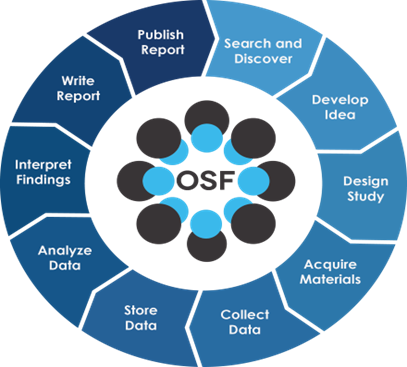
\includegraphics{img/osf-researchcycle.png}

\caption{\label{fig-osf-researchcycle}OSF Research Lifecycle}

\end{figure}%

\subsection{Open Science Framework
(OSF)}\label{open-science-framework-osf}

O material utilizado nesse módulo do curso segue de perto a proposta de
Olson et al. (2022), um \href{https://osf.io/yaqe8/}{projeto oficial do
COS} que possui recursos, modelos e práticas para ajudar os
pesquisadores a iniciar sua jornada \textbf{OSF}. Claro que ele foi
adaptado para nossos fins, principalmente, em decorrência do tempo
destinado ao módulo.

\begin{tcolorbox}[enhanced jigsaw, left=2mm, arc=.35mm, rightrule=.15mm, opacitybacktitle=0.6, breakable, toprule=.15mm, bottomrule=.15mm, leftrule=.75mm, colframe=quarto-callout-tip-color-frame, coltitle=black, bottomtitle=1mm, titlerule=0mm, toptitle=1mm, title=\textcolor{quarto-callout-tip-color}{\faLightbulb}\hspace{0.5em}{Bifurcando ou duplicando um projeto}, opacityback=0, colbacktitle=quarto-callout-tip-color!10!white, colback=white]

Você sabia que é possível executar um ``\emph{forking}'' (criar uma
cópia do projeto existente) ou ``\emph{duplicate as template}''
(duplicar apenas a estrutura do projeto e seus componentes) de um
projeto público no OSF?

Você que se interessa em iniciar seu próprio projeto OSF com um modelo,
pode criar sua própria duplicata do projeto Olson et al. (2022) para
começar!

Neste \href{https://osf.io/yaqe8/}{projeto}, existem templates e
recursos básicos para diversos casos de uso encontrados no OSF;
coordenação de equipes de pesquisa, planejamento de gerenciamento de
dados, documentos reprodutíveis e até mesmo gerenciamento de cursos.

\end{tcolorbox}

Para os alunos que desejam uma leitura sobre o \textbf{OSF} na prática,
indico os artigos de Sullivan, DeHaven, and Mellor (2019) e Soderberg
(2018). Apesar de o leitor poder encontrar \emph{prints} das telas da
plataforma desatualizadas, esses dois artigos podem ser um bom começo
para entender a lógica da plataforma. E \emph{off course}, recomendo
fortemente você dar uma olhada no
\href{https://help.osf.io/article/342-getting-started-on-the-osf}{suporte
do \textbf{OSF}}, onde podemos encontrar vídeos introdutórios
excelentes.

Esse curso poderia ter sido concebido e gerenciado dentro do
\textbf{OSF}, no entanto, devido a proposta de apresentarmos também o
\href{https://phdpablo.github.io/curso-open-science/05-git.html}{Git/Github}
e sua integração com documentos reprodutíveis no
\href{https://phdpablo.github.io/curso-open-science/06-quarto.html}{RStudio/Quarto}
(como esse que está lendo 😁), optamos por priorizar o repositório do
Github. Por isso, que também nesse módulo passamos pelo
\href{https://phdpablo.github.io/curso-open-science/00-prework.html\#sec-zenodoprework}{Zenodo},
que integra com o Github e tem a capacidade de gerar DOIs para as
versões dos repositórios.

\begin{tcolorbox}[enhanced jigsaw, left=2mm, arc=.35mm, rightrule=.15mm, opacitybacktitle=0.6, breakable, toprule=.15mm, bottomrule=.15mm, leftrule=.75mm, colframe=quarto-callout-note-color-frame, coltitle=black, bottomtitle=1mm, titlerule=0mm, toptitle=1mm, title=\textcolor{quarto-callout-note-color}{\faInfo}\hspace{0.5em}{@sullivan2019 \emph{Reading Note} (Tip~\ref{tip-prompt})}, opacityback=0, colbacktitle=quarto-callout-note-color!10!white, colback=white]

O artigo apresenta um protocolo para a implementação de práticas de
Ciência Aberta (CA), com foco no uso do Open Science Framework (OSF). As
principais ideias do texto são as seguintes:

\begin{itemize}
\item
  A CA é um movimento que promove a transparência, a reprodutibilidade e
  a acessibilidade dos resultados de pesquisa;
\item
  As práticas de CA podem contribuir para a melhoria da qualidade da
  pesquisa científica, tornando-a mais confiável e robusta;
\item
  O OSF é uma plataforma gratuita e de código aberto que pode ser usada
  para implementar práticas de CA;
\end{itemize}

O protocolo apresentado no texto fornece instruções passo a passo para
as seguintes práticas de CA:

\begin{itemize}
\item
  \textbf{Planejamento de gerenciamento de dados}: O planejamento de
  gerenciamento de dados é essencial para garantir que os dados de
  pesquisa sejam armazenados, organizados e gerenciados de forma
  eficiente e eficaz. O OSF fornece ferramentas para ajudar os
  pesquisadores a planejar e implementar seus planos de gerenciamento de
  dados.
\item
  \textbf{Pré-registro de estudos}: O pré-registro de estudos é uma
  prática que consiste em publicar um plano de pesquisa antes de iniciar
  o estudo. Isso ajuda a garantir que o estudo seja realizado de forma
  objetiva e transparente. O OSF fornece um recurso para pré-registrar
  estudos.
\item
  \textbf{Controle de versão}: O controle de versão é uma prática que
  consiste em rastrear as alterações feitas em arquivos de texto. Isso
  ajuda a garantir que os resultados de pesquisa sejam reprodutíveis e
  que as alterações feitas nos dados sejam rastreáveis. O OSF fornece
  ferramentas para gerenciar o controle de versão de arquivos de
  pesquisa.
\item
  \textbf{Compartilhamento de dados e materias}: O compartilhamento de
  dados e materiais de pesquisa é uma prática importante para aumentar a
  transparência e a reprodutibilidade da pesquisa. O OSF fornece um
  repositório para compartilhar dados e materiais de pesquisa.
\item
  \textbf{Publicação de pré-impressões}: As pré-impressões são versões
  preliminares de artigos científicos que são publicadas online antes de
  serem revisados por pares. As pré-impressões podem ajudar a acelerar a
  divulgação da pesquisa e a promover o debate científico. O OSF fornece
  um repositório para publicar pré-impressões.
\end{itemize}

O artigo fornece informações valiosas para os pesquisadores que desejam
implementar práticas de CA. O protocolo apresentado pode ser usado como
um guia para implementar essas práticas de forma eficaz.

\end{tcolorbox}

\bookmarksetup{startatroot}

\section{Gerenciamento de Referências e Bibliotecas}\label{sec-zotero}

\bookmarksetup{startatroot}

\section{Gestão de Dados e Projetos}\label{sec-project}

\bookmarksetup{startatroot}

\section{Controle de versão}\label{sec-git}

\bookmarksetup{startatroot}

\section{Documentos Reprodutíveis}\label{sec-quarto}

\bookmarksetup{startatroot}

\section{Controle de Ambiente (Containers)}\label{sec-docker}

\bookmarksetup{startatroot}

\section{IA Aplicada à Pesquisa Científica}\label{sec-AI}

\bookmarksetup{startatroot}

\section*{Referências}\label{referuxeancias}
\addcontentsline{toc}{section}{Referências}

\markboth{Referências}{Referências}

\phantomsection\label{refs}
\begin{CSLReferences}{1}{0}
\bibitem[\citeproctext]{ref-albano2023}
Albano, Cláudio Sonáglio, Paula de Oliveira Pedroso, and Doriedson
Oliveira Caetano. 2023. {``Ci{ê}ncia {Aberta}: {Um Panorama} Sobre as
{Publica{ç}{õ}es} No {Cen{á}rio Brasileiro}.''} \emph{Saber
Cient{í}fico} 12 (1): 1--12.

\bibitem[\citeproctext]{ref-baker2023}
Baker, Daniel H, Mareike Berg, Kirralise Hansford, Bartholomew Patrick
Anselm Quinn, Federico Gabriele Segala, and Erin English. 2023.
{``{ReproduceMe}: Lessons from a Pilot Project on Computational
Reproducibility.''} Preprint. PsyArXiv.
\url{https://doi.org/10.31234/osf.io/k8d4u}.

\bibitem[\citeproctext]{ref-baker2016}
Baker, Monya. 2016. {``1,500 Scientists Lift the Lid on
Reproducibility.''} \emph{Nature} 533 (7604): 452--54.
\url{https://doi.org/10.1038/533452a}.

\bibitem[\citeproctext]{ref-bernard2023}
Bernard, Christophe. 2023. {``Stop {Reproducing} the {Reproducibility
Crisis}.''} \emph{Eneuro} 10 (2): ENEURO.0032--23.2023.
\url{https://doi.org/10.1523/ENEURO.0032-23.2023}.

\bibitem[\citeproctext]{ref-bezjak2018}
Bezjak, Sonja, April Clyburne-Sherin, Philipp Conzett, Pedro Fernandes,
Edit Görögh, Kerstin Helbig, Bianca Kramer, et al. 2018. \emph{Open
{Science Training Handbook}}. Zenodo.
\url{https://doi.org/10.5281/ZENODO.1212496}.

\bibitem[\citeproctext]{ref-caballero-rivero2019}
Caballero-Rivero, Alejandro, Nancy Sánchez-Tarragó, and Raimundo Nonato
Macedo dos Santos. 2019. {``{Pr{á}ticas de Ci{ê}ncia Aberta da
comunidade acad{ê}mica brasileira: estudo a partir da produ{ç}{ã}o
cient{í}fica}.''} \emph{Transinforma{ç}{ã}o} 31 (November): e190029.
\url{https://doi.org/10.1590/2318-0889201931e190029}.

\bibitem[\citeproctext]{ref-chopik2018}
Chopik, William J., Ryan H. Bremner, Andrew M. Defever, and Victor N.
Keller. 2018. {``How (and {Whether}) to {Teach Undergraduates About} the
{Replication Crisis} in {Psychological Science}.''} \emph{Teaching of
Psychology} 45 (2): 158--63.
\url{https://doi.org/10.1177/0098628318762900}.

\bibitem[\citeproctext]{ref-crrs2019}
Committee on Reproducibility and Replicability in Science, Board on
Behavioral, Cognitive, and Sensory Sciences, Committee on National
Statistics, Division of Behavioral and Social Sciences and Education,
Nuclear and Radiation Studies Board, Division on Earth and Life Studies,
Board on Mathematical Sciences and Analytics, et al. 2019.
\emph{Reproducibility and {Replicability} in {Science}}. Washington,
D.C.: National Academies Press. \url{https://doi.org/10.17226/25303}.

\bibitem[\citeproctext]{ref-cruwell2019}
Crüwell, Sophia, Johnny Van Doorn, Alexander Etz, Matthew C. Makel,
Hannah Moshontz, Jesse C. Niebaum, Amy Orben, Sam Parsons, and Michael
Schulte-Mecklenbeck. 2019. {``Seven {Easy Steps} to {Open Science}: {An
Annotated Reading List}.''} \emph{Zeitschrift f{ü}r Psychologie} 227
(4): 237--48. \url{https://doi.org/10.1027/2151-2604/a000387}.

\bibitem[\citeproctext]{ref-dogucu2022}
Dogucu, Mine, and Mine Çetinkaya-Rundel. 2022. {``Tools and
{Recommendations} for {Reproducible Teaching}.''} \emph{Journal of
Statistics and Data Science Education} 30 (3): 251--60.
\url{https://doi.org/10.1080/26939169.2022.2138645}.

\bibitem[\citeproctext]{ref-EU2017}
European Commission. Directorate General for Research and Innovation.
2017. \emph{Providing Researchers with the Skills and Competencies They
Need to Practise {Open Science}.} LU: Publications Office.
\url{https://data.europa.eu/doi/10.2777/121253}.

\bibitem[\citeproctext]{ref-fanelli2018}
Fanelli, Daniele. 2018. {``Is Science Really Facing a Reproducibility
Crisis, and Do We Need It To?''} \emph{Proceedings of the National
Academy of Sciences} 115 (11): 2628--31.
\url{https://doi.org/10.1073/pnas.1708272114}.

\bibitem[\citeproctext]{ref-freedman2015}
Freedman, Leonard P., Iain M. Cockburn, and Timothy S. Simcoe. 2015.
{``The {Economics} of {Reproducibility} in {Preclinical Research}.''}
\emph{PLOS Biology} 13 (6): e1002165.
\url{https://doi.org/10.1371/journal.pbio.1002165}.

\bibitem[\citeproctext]{ref-heinz2024}
Heinz, Michele, and Miranda Miranda. 2024. {``Ci{ê}ncia {Aberta}:
Argumentos e Desafios Para Sua Legitima{ç}{ã}o Cient{í}fica.''} \emph{Em
Quest{ã}o} 30. \url{https://doi.org/10.1590/1808-5245.30.135618}.

\bibitem[\citeproctext]{ref-janz2015}
Janz, Nicole. 2015. {``Bringing the {Gold Standard} into the
{Classroom}: {Replication} in {University Teaching}.''}
\emph{International Studies Perspectives}, March, n/a--.
\url{https://doi.org/10.1111/insp.12104}.

\bibitem[\citeproctext]{ref-mcaleer2022}
McAleer, Phil, Niamh Stack, Heather Woods, Lisa Marie DeBruine, Helena
Paterson, Emily Nordmann, Carolina Ellen Kuepper-Tetzel, and Dale J.
Barr. 2022. {``Embedding {Data Skills} in {Research Methods Education}:
{Preparing Students} for {Reproducible Research}.''} Preprint. PsyArXiv.
\url{https://doi.org/10.31234/osf.io/hq68s}.

\bibitem[\citeproctext]{ref-mendes-da-silva2023}
Mendes-Da-Silva, Wesley. 2023. {``What {Lectures} and {Research} in
{Business Management Need} to {Know About Open Science}.''}
\emph{Revista de Administra{ç}{ã}o de Empresas} 63 (4): e0000--0033.
\url{https://doi.org/10.1590/s0034-759020230408x}.

\bibitem[\citeproctext]{ref-munafo2017}
Munafò, Marcus R., Brian A. Nosek, Dorothy V. M. Bishop, Katherine S.
Button, Christopher D. Chambers, Nathalie Percie Du Sert, Uri Simonsohn,
Eric-Jan Wagenmakers, Jennifer J. Ware, and John P. A. Ioannidis. 2017.
{``A Manifesto for Reproducible Science.''} \emph{Nature Human
Behaviour} 1 (1): 0021. \url{https://doi.org/10.1038/s41562-016-0021}.

\bibitem[\citeproctext]{ref-neto2016}
Neto, Silvio Carvalho, John Willinsky, and Juan Pablo Alperin. 2016.
{``Measuring, Rating, Supporting, and Strengthening Open Access
Scholarly Publishing in {Brazil}.''} \emph{Education Policy Analysis
Archives} 24 (May): 54--54. \url{https://doi.org/10.14507/epaa.24.2391}.

\bibitem[\citeproctext]{ref-olson2022}
Olson, Eric, Nicole Pfeiffer, Mark Call, and Daniel Steger. 2022.
{``Getting Started on OSF,''} August.
\url{https://doi.org/10.17605/OSF.IO/YAQE8}.

\bibitem[\citeproctext]{ref-protzko2023}
Protzko, John, Jon Krosnick, Leif Nelson, Brian A. Nosek, Jordan Axt,
Matt Berent, Nicholas Buttrick, et al. 2023. {``High Replicability of
Newly Discovered Social-Behavioural Findings Is Achievable.''}
\emph{Nature Human Behaviour}, November.
\url{https://doi.org/10.1038/s41562-023-01749-9}.

\bibitem[\citeproctext]{ref-rezende2020}
Rezende, Laura Vilela Rodrigues, and Ernest Abadal Falgueras. 2020.
{``Estado Da Arte Dos Marcos Regulat{ó}rios Brasileiros Rumo {à}
{Ci{ê}ncia Aberta}.''} \emph{Encontros Bibli: Revista Eletr{ô}nica de
Biblioteconomia e Ci{ê}ncia Da Informa{ç}{ã}o} 25 (September): 01--25.
\url{https://doi.org/10.5007/1518-2924.2020.e71370}.

\bibitem[\citeproctext]{ref-silva2019}
Silva, Fabiano Couto Corrêa Da, and Lúcia Da Silveira. 2019. {``O
Ecossistema Da {Ci{ê}ncia Aberta}.''} \emph{Transinforma{ç}{ã}o} 31:
e190001. \url{https://doi.org/10.1590/2318-0889201931e190001}.

\bibitem[\citeproctext]{ref-silveira2023}
Silveira, Lúcia Da, Nivaldo Calixto Ribeiro, Remedios Melero, Andrea
Mora-Campos, Daniel Fernando Piraquive-Piraquive, Alejandro Uribe
Tirado, Priscila Machado Borges Sena, et al. 2023. {``Taxonomia Da
{Ci{ê}ncia Aberta}: Revisada e Ampliada.''} \emph{Encontros Bibli:
Revista Eletr{ô}nica de Biblioteconomia e Ci{ê}ncia Da Informa{ç}{ã}o}
28 (June). \url{https://doi.org/10.5007/1518-2924.2023.e91712}.

\bibitem[\citeproctext]{ref-soderberg2018}
Soderberg, Courtney K. 2018. {``Using OSF to Share Data: A Step-by-Step
Guide.''} \emph{Advances in Methods and Practices in Psychological
Science} 1 (1): 115--20. \url{https://doi.org/10.1177/2515245918757689}.

\bibitem[\citeproctext]{ref-sullivan2019}
Sullivan, Ian, Alexander DeHaven, and David Mellor. 2019. {``Open and
Reproducible Research on Open Science Framework.''} \emph{Current
Protocols Essential Laboratory Techniques} 18 (1): e32.
\url{https://doi.org/10.1002/cpet.32}.

\bibitem[\citeproctext]{ref-toelch2018}
Toelch, Ulf, and Dirk Ostwald. 2018. {``Digital Open
Science---{Teaching} Digital Tools for Reproducible and Transparent
Research.''} \emph{PLOS Biology} 16 (7): e2006022.
\url{https://doi.org/10.1371/journal.pbio.2006022}.

\bibitem[\citeproctext]{ref-unesco2021}
UNESCO. 2021. {``{UNESCO Recommendation} on {Open Science}.''} UNESCO.
\url{https://doi.org/10.54677/MNMH8546}.

\bibitem[\citeproctext]{ref-vicente-saez2018}
Vicente-Saez, Ruben, and Clara Martinez-Fuentes. 2018. {``Open {Science}
Now: {A} Systematic Literature Review for an Integrated Definition.''}
\emph{Journal of Business Research} 88 (July): 428--36.
\url{https://doi.org/10.1016/j.jbusres.2017.12.043}.

\end{CSLReferences}



\end{document}
